\documentclass[round]{bioinfo}

\usepackage{color}
\newcommand{\cred}{\color{red}}

\usepackage{amstext}
\usepackage{url}
% \usepackage[colorlinks,citecolor=blue,linkcolor=red,urlcolor=blue]{hyperref}
\newcommand{\thefirstpage}{1} \newcommand{\thelastpage}{1}

\copyrightyear{2010}
\pubyear{2010}

\hyphenation{Bic-Over-lap-per}

\begin{document}

\firstpage{1}
\application{}
\title[ExpressionView]{ExpressionView -- an interactive viewer for
  modules identified in gene expression data}
\author[Andreas L\"uscher, G\'abor Cs\'ardi, Aitana Morton de
Lachapelle, Zolt\'an Kutalik, and Sven Bergmann]{Andreas
  L\"uscher$^{1*}$, G\'abor Cs\'ardi$^{1,2*}$, Aitana Morton de
  Lachapelle$^{1,2*}$, Zolt\'an Kutalik$^{1,2*}$,
  Bastian Peter$^{1,2}$
  and Sven Bergmann$^{1,2}$}
\address{
  $^{1}$Swiss Institute of Bioinformatics, Lausanne, Switzerland\\
  $^{2}$Department of Medical Genetics, University of Lausanne,
  Lausanne, Switzerland\\
  *: equal contribution
}

\history{Received on XXXXX; revised on XXXXX; accepted on XXXXX}

\editor{Associate Editor: XXXXXXX}

\maketitle

\begin{abstract}
\section{Summary:}
ExpressionView is an R package that provides an interactive graphical
environment to explore transcription modules identified in gene expression
data. A sophisticated ordering algorithm is used to present the
modules with the expression in a visually appealing layout that provides an intuitive
summary of the results. From this overview, the user can select
individual modules and access biologically relevant metadata
associated with them.

\section{Availability:}
%\href{http://www.unil.ch/cbg/ExpressionView}{R
%  package with open source license,
\url{http://www.unil.ch/cbg/ExpressionView}
%}

\section{Contact:} \href{Sven.Bergmann@unil.ch}{Sven.Bergmann@unil.ch}

\section{Supplementary information:}
Screenshots, tutorials and sample data sets can be found on the
ExpressionView \href{http://www.unil.ch/cbg/ExpressionView}{website}.
\end{abstract}

\vspace*{-9pt}
\section{Introduction}
Biclustering is an unsupervised data analysis method which is
frequently used to explore microarray data. Biclustering algorithms
process collections of expression profiles to identify groups of genes
co-expressed under some conditions (samples). We refer to such groups
as modules. While there is a multitude of biclustering software
available (for reviews  and comparisons
see~\cite{madeira04,ihmels04,prelic06}), packages with intuitive
interfaces that allow for an interactive exploration of the results
are sparse. 

Existing approaches include Bivisu~\citep{cheng07} and
BicOverlapper~\citep{santamaria08}. The former is an interactive
biclustering program that plots modules individually, making it
difficult to identify the relationship between the overlapping
modules. The latter is a novel tool for plotting overlapping modules,
yet in an abstract space. Our approach in ExpressionView is different,
as we use the usual gene-sample space and visualize all modules
together, on top of the reordered expression matrix. The reordering
ensures that the genes and samples that appear in the same module are
kept together.

\vspace*{-9pt}
\section{Package design and workflow}
With the ExpressionView package, bicluster analysis can be separated
into two parts. The first part involves finding the
modules in the data set with some algorithm, possibly running
enrichment analysis for the modules, and reordering the rows and
columns of the expression matrix according to the modules. This
part is typically done by a bioinformatician. The second part of the
analysis involves the visualization and interactive exploration of the
results. This part is typically done by researchers without extensive
programming knowledge.

The first part of ExpressionView is written in GNU
R~\citep{R} and contains an implementation of the matrix reordering
algorithm. The second part is an interactive visualization tool in
the form of an Adobe Flash applet, for which the user only needs a
Flash-enabled web browser.

This dual implementation has the advantage that all the power of the
GNU R environment and the BioConductor~\citep{gentleman04} packages
can be used for the analysis itself, e.g. all organisms that are (and
will be) supported by BioConductor are automatically supported by
ExpressionView. On the other hand, the exploration of the results does
not need any GNU R knowledge and in most cases no extra software needs to
be installed. See Fig.~\ref{fig:workflow} for a typical
ExpressionView workflow.

\begin{figure*}
\centering
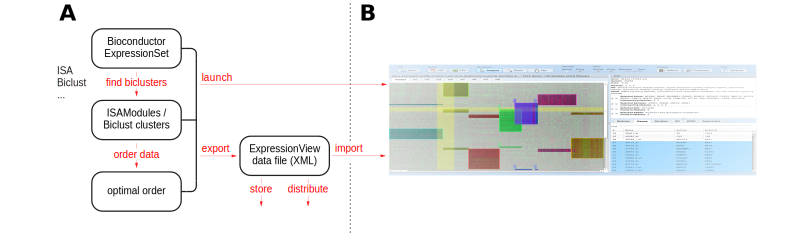
\includegraphics[width=0.7\linewidth]{fig1}
\caption{
  Workflow of ExpressionView, showing the two parts of the analysis.
  \textbf{(A)} These steps are performed by a bioinformatician,
  using GNU R. Starting from gene expression data in the form of a
  Bioconductor \textit{ExpressionSet}, the first step is finding the
  modules. In a second step, the rows and columns of the gene
  expression matrix are rearranged to produce an easily readable
  overview of the results. The last step consists of combining the
  gene expression data and its associated metadata, possibly including
  results of enrichment analysis, with the results
  from the biclustering and produce an ExpressionView data file.
  \textbf{(B)}~This file can be distributed and finally explored with
  the interactive Flash applet by the end-user. Please see the
  website for details on the data file format.}
\label{fig:workflow}
\end{figure*}

\vspace*{-9pt}
\subsection{Reordering genes and conditions}

% \subsection{Gene expression data and modules}
ExpressionView is designed to work with gene expression data in the
form of a Bioconductor \textit{ExpressionSet}. This class provides a
user-friendly way to access the actual gene expression matrix and its
associated metadata. ExpressionView can treat biclustering results obtained by the 
Iterative Signature Algorithm~\citep{bergmann03,csardi10} and any of 
the methods available in the Biclust package~\citep{kaiser08}. Since 
the structure of biclustering results is independent of the algorithm, 
an extension to other methods is straightforward.

To present the collection of possibly overlapping modules in a visually
appealing form, it is necessary to reorder the rows (conditions) and
columns (genes) of the gene expression matrix in such a way that
biclusters form contiguous
rectangles. Since it is in general impossible to find such an
arrangement for more than two mutually overlapping modules, we propose
here an approximate solution that optimizes the arrangement within the
original data, by maximizing the total area of the largest contiguous
module subsets. (An alternative would be to repeat rows and columns as
necessary~\citep{grothaus06}, but for many modules this results in
a very large expression matrix.)

This optimization task is an interesting problem on its own, which to
the best of our knowledge has not been studied in the literature.
We briefly outline our strategy here (see our website for details).
The reordering of the rows is independent from that of the columns,
so the same optimization method can be applied separately
to rows and columns. For a given order of the
elements (either genes or conditions), we compute for each module $i$ the
size of the largest contiguous sequence of elements (i.e. the maximal
number of neighboring elements $N^\text{max}_i$). Then, as a measure of the
quality ($Q$) of the order, we sum this quantity over all modules
($Q=\sum_i N^\text{max}_i$). To optimize $Q$, an initial sequence is calculated using
hierarchical clustering. Two operations are then applied to this: (1)
permutations that exchange two elements within a module and (2) shifts
of a sequence of multiple elements of the same module to a different position. We
use a greedy iterative scheme that performs these operations at
all possible positions and keeps the best new sequence if it improves
$Q$. The algorithm stops if after a given number of operations no
significant improvement of $Q$ is achieved.

We have studied a large number of perfectly orderable, but initially
scrambled, test cases. We find that the proposed algorithm finds an
order that recovers more than 99\% of the score of the optimal
solution and in most cases, it recovers the correct
alignment. For random samples, which are more representative for
actual gene expression data, the execution time increases polynomially
with the number of clusters $m$ as ${\mathcal O}(m^\alpha)$, where
$\alpha \in [1.6, 2]$, almost independently of the number of elements
$n$. For a given number of clusters, we find ${\mathcal O}(n^\alpha)$,
with $\alpha \in [2.5, 2.7]$.

Once the optimal order is determined, the program rearranges the gene
expression matrix accordingly and exports all the relevant information
into an XML file, that can be placed on a web-server or distributed by
email and then imported by the interactive viewer.

\subsection{Visualisation}

A screenshot of the viewer is shown in Fig.~\ref{fig:workflow}. The
interface is divided in two parts: On the left-hand side, the user
finds the gene expression data in the common heat map form, on top of
which the modules are overlaid. On the right-hand side, the metadata
associated with the expression data and the results of the
enrichment calculations for GO~\citep{ashburner00} categories and
KEGG~\citep{kanehisa04} pathways are shown. Wherever possible, these elements
are linked to the corresponding databases. The interface essentially
behaves as an image viewer, allowing the user to zoom and pan around
the expression data, getting instant feedback on the selected
item.

\section*{Acknowledgement}

\paragraph{Funding\textcolon} The authors are grateful to the Swiss
Institute of Bioinformatics, the Swiss National Science Foundation
(3100AO-116323/1) and the European Framework Project 6 (through
the EuroDia and AnEuploidy projects).

\paragraph{Conflict of interest\textcolon} none declared.

\vspace*{-9pt}
\bibliographystyle{natbib}
\bibliography{expressionview}

\end{document}
